\section[Выбор и обоснование средств реализации]{ВЫБОР И ОБОСНОВАНИЕ \\ СРЕДСТВ РЕАЛИЗАЦИИ}
\label{sec:choice}

В этом разделе рассматриваются различные аспекты реализации разрабатываемого веб-сервиса.

В подразделе~\ref{ssec:choice_opendata} перечислены требования, предъявляемые к открытым даннным
в целом и данным, которые будут предоставляться разрабатываемым веб-сервисом в частности.
Подраздел~\ref{ssec:choice_free_licenses} содержит информацию о видах свободных лицензий и различиях между ними.
В подразделе~\ref{ssec:choice_cms} находятся сведения о популярных системах управления контентом,
обсуждаются их достоинства и недостатки.
Подраздел~\ref{ssec:choice_db} содержит краткий обзор популярных реляционных СУБД,
распространяемых по свободной лицензии.
В подразделе~\ref{ssec:choice_web-server} обсуждаются вопросы выбора веб-сервера для выдачи контента пользователям.
Подраздел~\ref{ssec:choice_php_communication} содержит описание методов взаимодействия интерпретатора PHP с веб-сервером.

\subsection{Открытые данные}
\label{ssec:choice_opendata}

\textit{Открытые данные} --- концепция, отражающая идею о том, что определённые данные
должны быть свободно доступны для машиночитаемого использования и дальнейшей републикации без
ограничений авторского права, патентов и других механизмов контроля~\cite{wiki_opendata}.

Открытые данные характеризуется следующими признаками:
\begin{itemize}

\item
Доступность и читаемость: данные должны быть доступны целиком не дороже
разумной стоимости их воспроизведения; желательно через интернет.
Формат данных должен быть удобным для чтения и изменения.

\item
Повторное использование и распространение: данные должны предоставляться на условиях,
которые разрешают их повторное использование и распространение,
в том числе --- в комбинации с другими наборами данных.

\item
Всеобщее участие: каждый должен иметь возможность использовать и распространять данные.
Не должно быть дискриминации областей применения, людей или групп.
Например, ограничение «только для некоммерческого использования»,
которое запрещает «коммерческое» применение, или ограничение возможных областей применения
(к примеру, только в образовании), недопустимы.

\end{itemize}

Благодарю чёткому определению <<открытости>> есть возможность комбинировать данные
из различных источников~\cite{opendatahandbook_open_data}.

Освободить данные от ограничений авторского права можно с помощью свободных
лицензий~\cite{wiki_opendata}.

Данные, предоставляемые пользователям разрабатываемого сервиса, удовлетворяют требованиям, 
выдвигаемым к открытым данным.

\subsection{Выбор свободные лицензии}
\label{ssec:choice_free_licenses}

\paragraph{}
\textit{Свободная лицензия} --- такой лицензионный договор,
условия которого содержат разрешения пользователю от правообладателя
на конкретный перечень способов использования его произведения,
которые дают ему четыре важнейшие свободы:

\begin{itemize}
\item  
  свобода использовать произведение в любых целях, изучать его;
\item
  свобода создавать и распространять копии произведения;
\item
  свобода вносить в произведение изменения;
\item
  свобода публиковать и распространять такие изменённые производные произведения~\cite{wiki_free_license}.
\end{itemize}

\textit{Копилефт} --- обобщенный метод сделать продукт
(программа, текст, фото- или видеоматериал) свободным и потребовать,
чтобы все последующие измененные и дополненные версии этого продукта также оставались свободными~\cite{gnu_copyleft}.

Различают пермиссивные и копилефтные свободные лицензии.

\textit{Копилефтной лицензией} называется лицензия, использующая копилефт.

Наиболее известные копилефтные лицензии: универсальная общественная лицензия GNU, 
 лицензия свободной документации GNU, Creative Commons Attribution-Sharealike 2.0.

\textit{Пермиссивные лицензии на свободное ПО} --- лицензии на программное обеспечение,
которые практически не ограничивают свободу действий пользователей ПО и разработчиков,
работающих с исходным кодом.

В частности, пермиссивные лицензии сами по себе не ограничивают выбор лицензии для работ,
производных от работы с пермиссивной лицензией. Следовательно, пермиссивные лицензии не являются копилефтом.

Наиболее известные пермиссивные лицензии: лицензия BSD, лицензия MIT, Mozilla Public License, Creative Commons Attribution 2.0.

\paragraph{}
Исходный код разрабатываемого сервиса будет опубликован под копилефтной лицензией 
Creative Commons 3.0 ShareAlike Unported.

Перечислим её основные положения. Лицензия разрешает:
\begin{itemize}
\item копировать и распространять материал на любом носителе и в любом формате;
\item видоизменять и создавать новое, опираясь на этот материал, для любых целей, включая коммерческие.
\end{itemize}

Условия лицензии:
\begin{itemize}
\item требуется обеспечить соответствующее указание авторства, предоставить ссылку на лицензию,
  и обозначить изменения, если таковые были сделаны;
\item если исходный материал был переработан или взят за основу для производного произведения,
  требуется распространять переделанные части материала на условиях той же лицензии, 
  в соответствии с которой распространяется оригинал~\cite{cc_by_sa}.
\end{itemize}

Таким образом, лицензия, используемая разрабатываемым сервисом, является копилефтной. 

\subsection{Выбор системы управления контентом}
\label{ssec:choice_cms}

\paragraph{}
\textit{Система управления контентом (CMS)} --- информационная система или компьютерная программа,
используемая для обеспечения и организации совместного процесса создания,
редактирования и управления контентом~\cite{wiki_cms}.

\textit{Контент} --- все виды информации (как текстовой, так и мультимедийной: изображения, аудио, видео),
составляющей наполнение веб-сайта~\cite{wiki_content}.

Основные функции систем управления контентом:
\begin{itemize}
\item
  Создание --- предоставление авторам удобных и привычных средств создания контента.

\item
  Управление --- хранение контента в едином репозитории. 
  Это позволяет следить за версиями документов, контролировать, кто и когда их изменял, убеждаться,
  что каждый пользователь может изменить только тот раздел, за который он отвечает.
  Кроме того, обеспечивается интеграция с существующими информационными источниками и ИТ-системами.

\item
  Публикация --- автоматическое размещение контента на терминале пользователя. 
  Соответствующие инструменты автоматически приводят внешний вид страницы к дизайну всего сайта.

\item
  Представление --- дополнительные функции, позволяющие улучшить форму представления данных; например,
  можно строить навигацию по структуре репозитория~\cite{osp_cms_functions}.
\end{itemize}

Использование системы управления контентом позволяет существенно снизить время и затраты на разработку.

\paragraph{}
На рисунке~\ref{fig:cms_usage_dynamic} приведены данные об использования систем управления контентом в интернете за период
с 1 сентября 2011 по 19 сентября 2012 года. Рост кривой свидетельствует о росте популярности решений на 
основе систем управления контентом.

\begin{figure}[h]
  \centering
  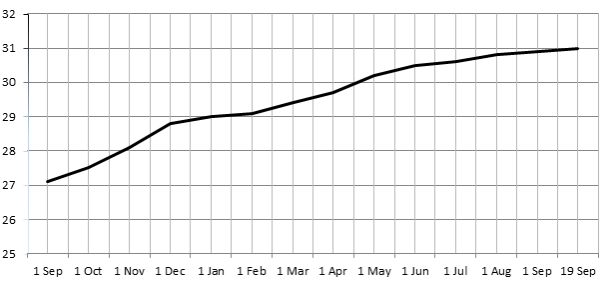
\includegraphics[width=150mm]{pic/dynamic_cms_usage.png}
  \caption{График использования систем управления контентом в интернете}
  \label{fig:cms_usage_dynamic}
\end{figure}

Соотношение использования систем управления контентом по состоянию на март 2014 года приведено
на рисунке~\ref{fig:cms_usage_stat}.

\begin{figure}[h]
  \centering
  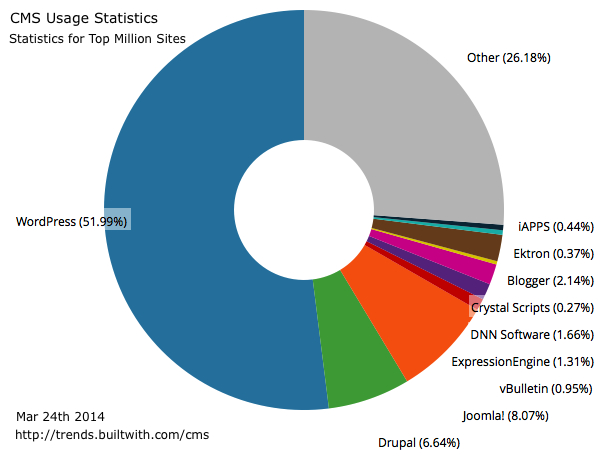
\includegraphics[width=100mm]{pic/cms_usage_statistics.png}
  \caption{Соотношение использования систем управления контентом}
  \label{fig:cms_usage_stat}
\end{figure}

Наиболее популярными решениями являются Wordpress (51{,}99\%), Joomla (8{,}07\%), Drupal 6{,}64\%).
Ограничим круг рассмотрения этими тремя CMS.

\paragraph{}
WordPress --- наиболее популярная система управления контентом:
более половины пользователей предпочитают именно WordPress.

Достоинства WordPress:
\begin{itemize}
\item
  наиболее широкий набор плагинов, тем, виджетов для галерей, форумов;
\item
  поддержка мультиязычности, различные каталоги, магазины;
\item
  поддержка WYSIWYG редактора текста;
\item
  технический опыт разработки не обязателен: панель администратора намного проще, чем в у конкурентов:
  PHP и CSS файлы можно редактировать непосредственно в ней.
\end{itemize}

Недостатки WordPress:
\begin{itemize}
\item
  данная система управления контентом изначально разрабатывалась для ведения блогов, новостных сайтов; 

\item
  возможны некоторые проблемы при установке,
  несмотря на распространённое мнение о самом лёгком процессе установки.
\end{itemize}

\paragraph{} 
Joomla представляет собой что-то среднее между обширными возможностями ориентированного на
разработчиков Drupal и простотой WordPress, но с более широкими возможностями для разработки.

Достоинства Joomla:
\begin{itemize}
\item
  несмотря на простоту в сравнении с Drupal, Joomla является полноценным инструментом для разработки;
\item
  поддержка протоколов контроля доступа (OpenID, LDAP, Gmail.com);
\item
  наличие удобной панели администратора с широким набором функций.
\end{itemize}

Недостатки Joomla:
\begin{itemize}
\item
  cистема довольно поверхностна и слаба, несмотря на всю универсальность;
\item
  больше платных плагинов и тем в сравнении с WordPress;
\end{itemize}

\paragraph{}
Около 7\% пользователей предпочитают Drupal. Разработчикам нравится его всеобъемлющая мощь
и дружественный разработчику интерфейс, который позволяет создавать сложные веб-сайты.

Достоинства Drupal:
\begin{itemize}
\item
  модули fields и views позволяют конструировать произвольные типы данных и их отображение;
\item
  модуль Taxonomy позволяет систематизировать контент по уровням, признакам и категориям;
\item
  Drupal имеет и большое и активное сообщество;
\end{itemize}

Недостатки Drupal:
\begin{itemize}
\item 
  из-за своей сложности Drupal определенно не подходит для неопытного пользователя;
\item
  Drupal требует прогрессивного технического оборудования,
  иначе могут возникнуть некоторые проблемы в плане производительности.
\end{itemize}

\paragraph{}
В качестве инструмента для разработки проектируемого веб-сервиса была выбрана система управления Drupal 7.0.
Выбор обусловлен следующими причинами:
\begin{itemize}
\item
  нестандартность функционала разрабатываемого сервиса;
\item
  богатый функционал системы управления контентом Drupal;
\item 
  Drupal распространяется под свободной лицензией GPLv3;
\end{itemize}  

\subsection{Выбор СУБД}
\label{ssec:choice_db}

Система управления контентом Drupal 7 изначально поддерживает следующие СУБД 
в качестве основного хранилища данных:
\begin{itemize} 
\item
  MySQL 5.0.15 и выше (рекомендуется);

\item
  PostgreSQL 8.3 и выше;

\item
  SQLite 3.3.7.
\end{itemize}

При подключении дополнительных модулей возможна интеграция с Microsoft SQL Server и Oracle,
а также с различными NoSQL решениями~\cite{drupal_database}.

Для реализации проектируемого веб-сервиса будет использоваться СУБД MySQL 5.5 по следующим причинам:
\begin{itemize}
\item
  это бесплатная СУБД, распространяемая под свободной лицензией для некоммерческого использования;
\item
  взаимодействие Drupal с ней является наиболее отлаженным;
\item
  она хорошо масштабируется и разработана для работы при большой частоте запросов;
\end{itemize}

\subsection{Выбор веб-сервера}
\label{ssec:choice_web-server}

В качестве кандидатов на роль веб-сервера, обрабатывающего запросы пользователей,
представлены варианты, перечисленные далее.

\begin{itemize}
  \item Apache --- свободный веб-сервер. Основными достоинствами Apache считаются надёжность и гибкость конфигурации.
    Он позволяет подключать внешние модули для предоставления данных, использовать 
    СУБД для аутентификации пользователей, модифицировать сообщения об ошибках и~т.~д. Поддерживает IPv6~\cite{wiki_apache}.

  \item Nginx --- простой, быстрый и надёжный сервер, не перегруженный функциями.
    Применение nginx целесообразно прежде всего для статических веб-сайтов
    и как прокси-сервера перед динамическими сайтами~\cite{wiki_nginx}.
\end{itemize}

В качестве веб-сервера для реализуемого веб-сервиса было выбран Apache, так как только этот сервер доступен
на веб-хостинге, на котором этот сервис будет размещаться.

\subsection{Выбор режима взаимодействия с PHP}
\label{ssec:choice_php_communication}

\paragraph{}
Система управления контентом Drupal написана на PHP, следовательно, для её использования необходимо связать
веб-сервер с интерпретатором PHP.

При использовании веб-сервера Apache это можно сделать двумя способами: PHP как модуль Apache и PHP как FastCGI.
Приведем характеристикку каждого из методов.

\paragraph{}
PHP, как модуль Apache. В данном случае для работы PHP используется модуль веб-сервера apache mod\_php.

Достоинства данного метода:
\begin{itemize}
\item
  cамая высокая скорость работы скриптов, по сравнению с другими методами (на больших количествах запросов);
\item
  простота работы, так как сервер сам обрабатывает скрипты;
\item
  наличие общего конфигурационного файла для всех скриптов (php.ini);
\item
  возможность задания переменных конфигурации PHP в конфигурационном файле web-сервера или средствами файла .htaccess.
\end{itemize}

Недостатки:
\begin{itemize}
\item все скрипты запускаются с правами с которым работает web-сервер, 
  тем самым если есть необходимость записи в какую либо директорию --- права доступа необходимо дать на неё всем,
  т.е. низкая безопасность;
\item
  в случае запуска сторонних приложений скриптами (например, почтовая рассылка), нет возможности идентифицировать пользователя,
  который запустил процесс;
\item
  излишняя нагрузка на web-сервер: аpache, занятый обработкой скриптов, может медленно отдавать другие статические данные;
\item
  ошибки в скриптах могут привести к неработоспособности всего web-сервера.
\end{itemize}

\paragraph{}
PHP, как FastCGI. При этом используется модуль Apache mod\_fastcgi,
скрипты передаются его средствами на вход интерпретатора PHP.

Достоинства данного метода:
\begin{itemize}
\item
  все скрипты выполняются с правами владельца домена;
\item
  возможность индивидуальной настройки PHP;
\item
  меньший расход оперативной памяти по сравнению с mod\_php;
\item
  ошибки в скриптах не приводят к падению веб-сервера в отличие от режима PHP как модуль apache;
\item
  За счет кэширования некоторых промежуточных данных скрипт не интерпретируется каждый раз при выполнении
  и достигается более высокая скорость по сравнению с PHP как CGI.
\end{itemize}

Как недостаток использования FastCGI можно отметить тот факт, что лишний процесс пользователя (php-cgi)
находится в памяти после первого обращения к процессу.

Недостатки:
\begin{itemize}
\item все скрипты запускаются с правами с которым работает web-сервер, 
  тем самым если есть необходимость записи в какую либо директорию --- права доступа необходимо дать на неё всем,
  т.е. низкая безопасность;
\item
  в случае запуска сторонних приложений скриптами (например, почтовая рассылка),
  нет возможности идентифицировать пользователя, который запустил процесс;
\item
  излишняя нагрузка на web-сервер: аpache, занятый обработкой скриптов, может медленно отдавать другие статические данные;
\item
  ошибки в скриптах могут привести к неработоспособности всего web-сервера~\cite{komtet_php_conf}.
\end{itemize}

\paragraph{}
Веб-хостинг, на котором будет размещаться разрабатываемый сервис, поддерживает только вариант использования PHP через FastCGI,
что однозначно определяет наш выбор.

\subsection{Результаты выбора средств реализации}
\label{ssec:choice_results}

В качестве средств реализации были выбраны следующие технологии:
\begin{itemize}
\item система управления контентом Drupal 7.0;
\item база данных MySQL 5.5;
\item веб-сервер Apache 2.2;
\item метод взаимодействия веб-сервера с интерпретатором PHP --- mod\_php.

\end{itemize}

Код и данные, предоставляемые пользователям разрабатываемого сервиса будут опубликованы 
под свободной лицензией Creative Commons Attribution-ShareAlike 3.0 Unported.